\chapter{\acrlong{rc}}

\section{Introduction}

\gls{rc} is a bio-inspired artificial recurrent neural network which is based on the \gls{esn} paradigm introduced by Herbert Jaeger in \cite{Jaeger2004}. This computation scheme is well suited for real-time data processing and for chaotic time series prediction\cite{Jaeger2004, JaegerH.2001Tesa, Lukoeviius2012}, and achieves state of the art performances in those domains, as well as in speech recognition\cite{Verstraeten2006, NIPS2010_4056, Jaeger2007}, nonlinear channel equalisation\cite{Jaeger2004} and financial forecasting \cite{financialTimeSeries}.\\

A \gls{rcer} is made of a large ensemble of interconnected neurons, which are merely entities carrying an activation level. The activation level  is updated according to the connection weights of the reservoir, or \emph{synaptic matrix} as it is referred to in the field of neural networks, and with a nonlinear function, called the \textit{activation function}. The nonlinear character is one of the main features making neural networks so powerful. Moreover, with a proper activation function, one can reach a saturation state, which mimics the behaviour of biological neurons. This is traditionally achieved using the \textit{sigmoid} function. Those principles are introduced in \cite[p.227-228]{bishop2006pattern} and in \cite[p.727-728]{russell2010artificial}.\\

\begin{figure}[h]
	\centering
	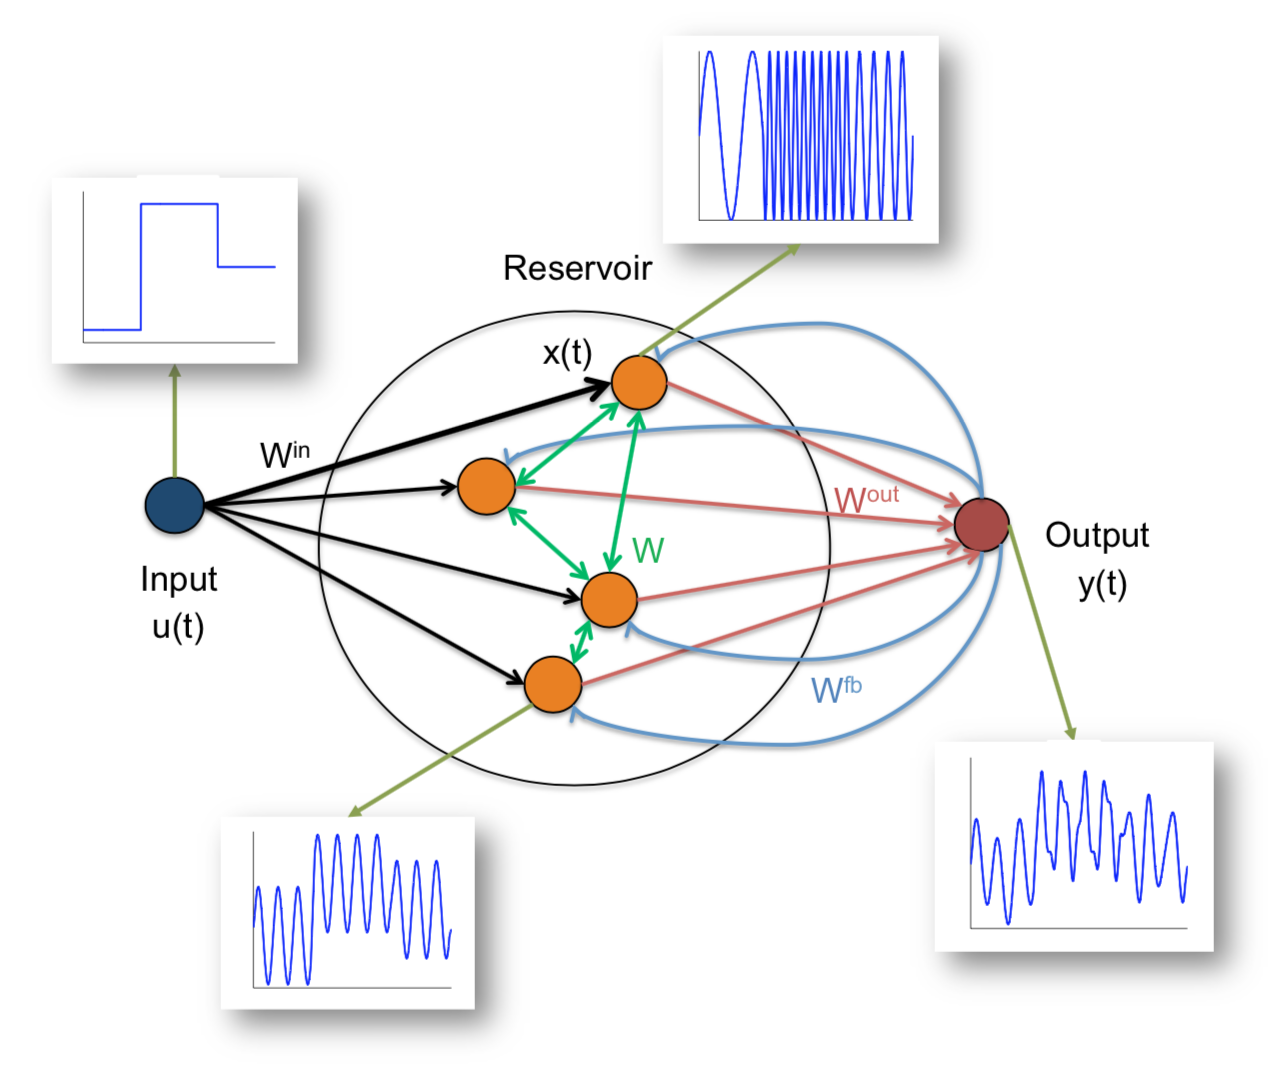
\includegraphics[width=.55\textwidth]{rc_principle.png}
	\caption{Principle scheme of a \acrshort{rcer} \cite{financialTimeSeries}}
	\label{rc_principle}
\end{figure}

The activation level of the neurons making up the reservoir characterise its state, which is time-dependent object. The neurons are interconnected in such a way that they influence the dynamic of each other, leading to a complicated evolution the state of the reservoir. What a first glance may seem to be a mathematical nightmare turns out to be the main advantage of \gls{rc}, making it so powerful. Indeed, by making the connection matrix as messy as possible, \textit{i.e.} by using randomness, breaking symmetries,... one notices that the effect of such a reservoir, when being fed a time-dependent signal, is to map it to a higher-dimensional functional space, the dimensionality being determined by the intrinsic dynamics of the neurons and depending on the richness of the connection matrix. Its link to \gls{esn} provides  \gls{rc} with another advantage compared to other computation schemes,  namely it has a memory of the input, thanks to the fact that the neurons are \textit{echoing} the effect of the input to one another. The output of the reservoir is obtained by adequately combining the neurons using the output matrix. These notions are summarised at the Figure \ref{rc_principle}.\\

